% shared preamble of the theory figures (white background, purple / black theme, sans-serif)
\documentclass[tikz,border=8pt]{standalone}
\usepackage[T1]{fontenc}
\usepackage[scaled=0.92]{helvet}
\renewcommand{\familydefault}{\sfdefault}
\usepackage{amsmath,amssymb}
\usepackage[helvet]{sfmath}
\usetikzlibrary{arrows.meta,calc,decorations.pathreplacing,positioning,backgrounds}
\definecolor{ink}{HTML}{1A1A1F}
\definecolor{cohesin}{HTML}{6A3DE8}
\definecolor{condensin}{HTML}{1BAF7A}
\definecolor{fwd}{HTML}{D1303F}      % CTCF pointing right
\definecolor{rev}{HTML}{2B62D9}      % CTCF pointing left
\definecolor{panel}{HTML}{F8F6FD}
\definecolor{panelline}{HTML}{E3DDF5}
\tikzset{
  fiber/.style={line width=2.1pt,ink,line cap=round,line join=round},
  halo/.style={line width=6pt,white,line cap=round},
  lab/.style={font=\small,text=ink},
  note/.style={font=\footnotesize,text=ink!60},
  hd/.style={font=\bfseries\small,text=ink,anchor=west},
  leader/.style={line width=0.6pt,ink!45},
}
% soft panel, numbered badge, heading
\newcommand{\panelbg}[4]{\draw[rounded corners=9pt,fill=panel,draw=panelline,line width=0.9pt] (#1,#2) rectangle (#3,#4);}
\newcommand{\badge}[3]{\fill[ink] (#1,#2) circle (0.21);\node[white,font=\bfseries\footnotesize] at (#1,#2) {#3};}
% CTCF: a protein on the fibre carrying an arrow that gives the motif direction (f = right, r = left)
\newcommand{\protf}[2]{\draw[rounded corners=3.5pt,line width=0.6pt,draw=fwd!65!black,fill=fwd] (#1-0.3,#2-0.19) rectangle (#1+0.3,#2+0.19);
  \draw[white,line width=1.5pt,-{Stealth[length=3.4pt,width=4.4pt]}] (#1-0.15,#2)--(#1+0.16,#2);}
\newcommand{\protr}[2]{\draw[rounded corners=3.5pt,line width=0.6pt,draw=rev!65!black,fill=rev] (#1-0.3,#2-0.19) rectangle (#1+0.3,#2+0.19);
  \draw[white,line width=1.5pt,-{Stealth[length=3.4pt,width=4.4pt]}] (#1+0.15,#2)--(#1-0.16,#2);}
\newcommand{\prot}[3]{\csname prot#3\endcsname{#1}{#2}}
% ring seen at an angle, drawn as a tube (dark outline, light core); back half and front half
\newcommand{\ringpart}[5]{\draw[line width=4.6pt,#3!80!black,line cap=round] ([shift={(#1,#2)}]#4:0.55 and 0.21) arc[start angle=#4,end angle=#5,x radius=0.55,y radius=0.21];
  \draw[line width=2.4pt,#3!55!white,line cap=round] ([shift={(#1,#2)}]#4:0.55 and 0.21) arc[start angle=#4,end angle=#5,x radius=0.55,y radius=0.21];}
\newcommand{\ringback}[3]{\ringpart{#1}{#2}{#3}{180}{0}}
\newcommand{\ringfront}[3]{\ringpart{#1}{#2}{#3}{180}{360}}
% smooth loop whose foot (ring) is at (cx,y0): half-width W, height H, ring colour
\newcommand{\lloop}[5]{%
  \ringback{#1}{#2}{#5}%
  \draw[fiber] (#1-0.3,#2) .. controls (#1-0.3,#2+0.25*#4) and (#1-#3,#2+0.2*#4) .. (#1-#3,#2+0.55*#4)
     .. controls (#1-#3,#2+0.95*#4) and (#1-0.5*#3,#2+#4) .. (#1,#2+#4)
     .. controls (#1+0.5*#3,#2+#4) and (#1+#3,#2+0.95*#4) .. (#1+#3,#2+0.55*#4)
     .. controls (#1+#3,#2+0.2*#4) and (#1+0.3,#2+0.25*#4) .. (#1+0.3,#2);%
  \ringfront{#1}{#2}{#5}}
% gently undulating fibre from x0 to the loop foot at cx (height y0), and from x1
\newcommand{\base}[4]{%
  \draw[fiber] plot[smooth] coordinates {(#1,0.05) (#1+0.35*#3-0.35*#1,-0.05) (#3-1.4,0.04)} .. controls (#3-0.6,0.02) and (#3-0.3,0.05) .. (#3-0.3,#4);
  \draw[fiber] plot[smooth] coordinates {(#2,-0.05) (#2-0.35*#2+0.35*#3,0.05) (#3+1.4,-0.04)} .. controls (#3+0.6,-0.02) and (#3+0.3,0.05) .. (#3+0.3,#4);}
% stop sign for a blocked leg and a leg arrow
\newcommand{\stopbar}[3]{\draw[#3,line width=2.4pt,line cap=round] (#1,#2-0.2)--(#1,#2+0.2);}
\newcommand{\legarrow}[3]{\draw[cohesin,line width=1.6pt,-{Stealth[length=5pt,width=6pt]},line cap=round] (#1,#3)--(#2,#3);}

\definecolor{A}{HTML}{D1303F}\definecolor{B}{HTML}{5B4FD6}
\tikzset{ln/.style={line width=0.7pt,ink!45},cur/.style={line width=1.8pt,cohesin},thin/.style={line width=0.9pt},
  mv/.style={line width=1.2pt,ink!70,-{Stealth[length=5pt,width=6pt]}},box/.style={rounded corners=5pt,draw=cohesin!70,fill=white,line width=0.9pt,align=center,font=\small,text=ink,inner sep=4pt}}
\begin{document}
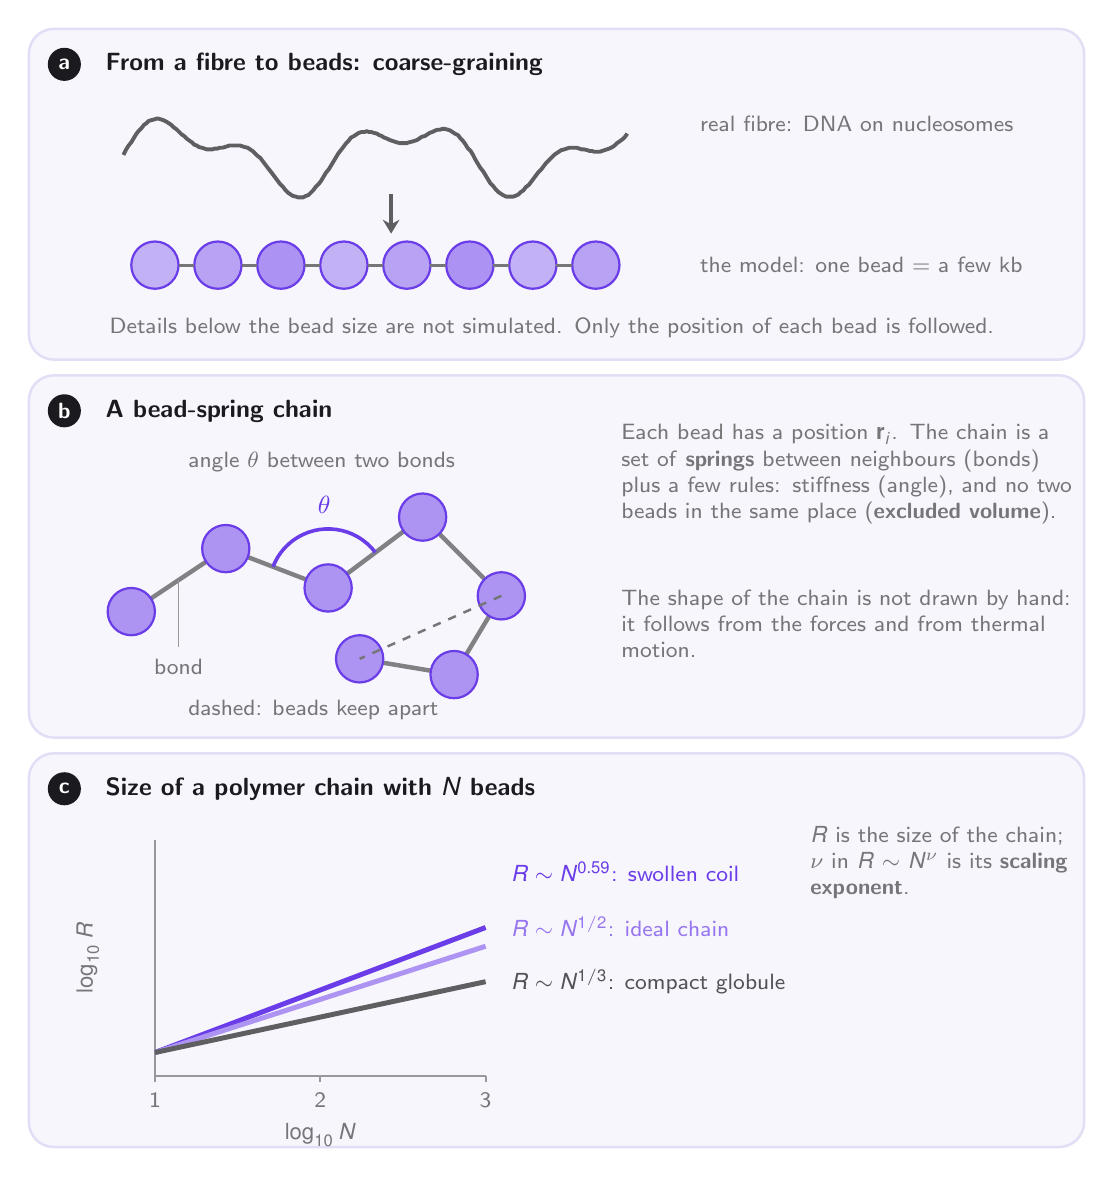
\begin{tikzpicture}
  \panelbg{0}{8.4}{13.4}{12.6}\badge{0.45}{12.15}{a}\node[hd] at (0.85,12.15) {From a fibre to beads: coarse-graining};
  \panelbg{0}{3.6}{13.4}{8.2}\badge{0.45}{7.749999999999999}{b}\node[hd] at (0.85,7.749999999999999) {A bead-spring chain};
  \panelbg{0}{-1.6}{13.4}{3.4}\badge{0.45}{2.9499999999999997}{c}\node[hd] at (0.85,2.9499999999999997) {Size of a polymer chain with $N$ beads};
  \draw[line width=1.4pt,ink!70] (1.20,11.00) -- (1.23,11.06) -- (1.26,11.11) -- (1.30,11.16) -- (1.33,11.21) -- (1.36,11.26) -- (1.39,11.30) -- (1.43,11.34) -- (1.46,11.38) -- (1.49,11.40) -- (1.52,11.43) -- (1.55,11.44) -- (1.59,11.45) -- (1.62,11.46) -- (1.65,11.46) -- (1.68,11.45) -- (1.71,11.44) -- (1.75,11.42) -- (1.78,11.40) -- (1.81,11.38) -- (1.84,11.35) -- (1.88,11.32) -- (1.91,11.29) -- (1.94,11.26) -- (1.97,11.24) -- (2.00,11.21) -- (2.04,11.18) -- (2.07,11.16) -- (2.10,11.13) -- (2.13,11.12) -- (2.16,11.10) -- (2.20,11.09) -- (2.23,11.08) -- (2.26,11.07) -- (2.29,11.07) -- (2.33,11.07) -- (2.36,11.08) -- (2.39,11.08) -- (2.42,11.09) -- (2.45,11.09) -- (2.49,11.10) -- (2.52,11.11) -- (2.55,11.12) -- (2.58,11.12) -- (2.62,11.12) -- (2.65,11.12) -- (2.68,11.12) -- (2.71,11.11) -- (2.74,11.10) -- (2.78,11.09) -- (2.81,11.07) -- (2.84,11.05) -- (2.87,11.02) -- (2.90,10.99) -- (2.94,10.96) -- (2.97,10.92) -- (3.00,10.88) -- (3.03,10.84) -- (3.07,10.79) -- (3.10,10.75) -- (3.13,10.71) -- (3.16,10.67) -- (3.19,10.63) -- (3.23,10.59) -- (3.26,10.55) -- (3.29,10.52) -- (3.32,10.50) -- (3.35,10.48) -- (3.39,10.47) -- (3.42,10.46) -- (3.45,10.46) -- (3.48,10.46) -- (3.52,10.48) -- (3.55,10.49) -- (3.58,10.52) -- (3.61,10.55) -- (3.64,10.59) -- (3.68,10.63) -- (3.71,10.67) -- (3.74,10.72) -- (3.77,10.77) -- (3.81,10.82) -- (3.84,10.87) -- (3.87,10.92) -- (3.90,10.97) -- (3.93,11.02) -- (3.97,11.07) -- (4.00,11.11) -- (4.03,11.15) -- (4.06,11.18) -- (4.09,11.22) -- (4.13,11.24) -- (4.16,11.26) -- (4.19,11.28) -- (4.22,11.29) -- (4.26,11.29) -- (4.29,11.30) -- (4.32,11.29) -- (4.35,11.29) -- (4.38,11.28) -- (4.42,11.27) -- (4.45,11.25) -- (4.48,11.24) -- (4.51,11.22) -- (4.54,11.21) -- (4.58,11.19) -- (4.61,11.18) -- (4.64,11.17) -- (4.67,11.16) -- (4.71,11.15) -- (4.74,11.15) -- (4.77,11.15) -- (4.80,11.15) -- (4.83,11.16) -- (4.87,11.17) -- (4.90,11.18) -- (4.93,11.19) -- (4.96,11.21) -- (4.99,11.23) -- (5.03,11.24) -- (5.06,11.26) -- (5.09,11.28) -- (5.12,11.29) -- (5.16,11.31) -- (5.19,11.32) -- (5.22,11.32) -- (5.25,11.33) -- (5.28,11.33) -- (5.32,11.32) -- (5.35,11.31) -- (5.38,11.29) -- (5.41,11.27) -- (5.45,11.25) -- (5.48,11.21) -- (5.51,11.18) -- (5.54,11.14) -- (5.57,11.09) -- (5.61,11.05) -- (5.64,11.00) -- (5.67,10.94) -- (5.70,10.89) -- (5.73,10.84) -- (5.77,10.79) -- (5.80,10.74) -- (5.83,10.69) -- (5.86,10.64) -- (5.90,10.60) -- (5.93,10.56) -- (5.96,10.53) -- (5.99,10.51) -- (6.02,10.49) -- (6.06,10.47) -- (6.09,10.47) -- (6.12,10.47) -- (6.15,10.47) -- (6.18,10.48) -- (6.22,10.50) -- (6.25,10.53) -- (6.28,10.55) -- (6.31,10.59) -- (6.35,10.62) -- (6.38,10.66) -- (6.41,10.70) -- (6.44,10.74) -- (6.47,10.78) -- (6.51,10.82) -- (6.54,10.86) -- (6.57,10.90) -- (6.60,10.93) -- (6.64,10.97) -- (6.67,11.00) -- (6.70,11.02) -- (6.73,11.04) -- (6.76,11.06) -- (6.80,11.07) -- (6.83,11.08) -- (6.86,11.09) -- (6.89,11.09) -- (6.92,11.09) -- (6.96,11.09) -- (6.99,11.08) -- (7.02,11.07) -- (7.05,11.07) -- (7.09,11.06) -- (7.12,11.05) -- (7.15,11.05) -- (7.18,11.04) -- (7.21,11.04) -- (7.25,11.04) -- (7.28,11.05) -- (7.31,11.06) -- (7.34,11.07) -- (7.37,11.08) -- (7.41,11.10) -- (7.44,11.12) -- (7.47,11.15) -- (7.50,11.17) -- (7.54,11.20) -- (7.57,11.23) -- (7.60,11.27);
  \node[note,anchor=west] at (8.4,11.4) {real fibre: DNA on nucleosomes};
  \fill[cohesin!40] (1.60,9.6) circle (0.3);\draw[cohesin,line width=0.8pt] (1.60,9.6) circle (0.3);
  \fill[cohesin!48] (2.40,9.6) circle (0.3);\draw[cohesin,line width=0.8pt] (2.40,9.6) circle (0.3);
  \draw[ink!60,line width=1pt] (1.90,9.6)--(2.10,9.6);
  \fill[cohesin!56] (3.20,9.6) circle (0.3);\draw[cohesin,line width=0.8pt] (3.20,9.6) circle (0.3);
  \draw[ink!60,line width=1pt] (2.70,9.6)--(2.90,9.6);
  \fill[cohesin!40] (4.00,9.6) circle (0.3);\draw[cohesin,line width=0.8pt] (4.00,9.6) circle (0.3);
  \draw[ink!60,line width=1pt] (3.50,9.6)--(3.70,9.6);
  \fill[cohesin!48] (4.80,9.6) circle (0.3);\draw[cohesin,line width=0.8pt] (4.80,9.6) circle (0.3);
  \draw[ink!60,line width=1pt] (4.30,9.6)--(4.50,9.6);
  \fill[cohesin!56] (5.60,9.6) circle (0.3);\draw[cohesin,line width=0.8pt] (5.60,9.6) circle (0.3);
  \draw[ink!60,line width=1pt] (5.10,9.6)--(5.30,9.6);
  \fill[cohesin!40] (6.40,9.6) circle (0.3);\draw[cohesin,line width=0.8pt] (6.40,9.6) circle (0.3);
  \draw[ink!60,line width=1pt] (5.90,9.6)--(6.10,9.6);
  \fill[cohesin!48] (7.20,9.6) circle (0.3);\draw[cohesin,line width=0.8pt] (7.20,9.6) circle (0.3);
  \draw[ink!60,line width=1pt] (6.70,9.6)--(6.90,9.6);
  \node[note,anchor=west] at (8.4,9.6) {the model: one bead = a few kb};
  \draw[mv] (4.6,10.5)--(4.6,10.0);
  \node[note,text width=11.8cm,anchor=north west] at (0.9,9.05) {Details below the bead size are not simulated. Only the position of each bead is followed.};
  \draw[ink!55,line width=1.6pt] (1.3,5.2)--(2.5,6.0);
  \draw[ink!55,line width=1.6pt] (2.5,6.0)--(3.8,5.5);
  \draw[ink!55,line width=1.6pt] (3.8,5.5)--(5.0,6.4);
  \draw[ink!55,line width=1.6pt] (5.0,6.4)--(6.0,5.4);
  \draw[ink!55,line width=1.6pt] (6.0,5.4)--(5.4,4.4);
  \draw[ink!55,line width=1.6pt] (5.4,4.4)--(4.2,4.6);
  \fill[cohesin!55] (1.3,5.2) circle (0.3);\draw[cohesin,line width=0.8pt] (1.3,5.2) circle (0.3);
  \fill[cohesin!55] (2.5,6.0) circle (0.3);\draw[cohesin,line width=0.8pt] (2.5,6.0) circle (0.3);
  \fill[cohesin!55] (3.8,5.5) circle (0.3);\draw[cohesin,line width=0.8pt] (3.8,5.5) circle (0.3);
  \fill[cohesin!55] (5.0,6.4) circle (0.3);\draw[cohesin,line width=0.8pt] (5.0,6.4) circle (0.3);
  \fill[cohesin!55] (6.0,5.4) circle (0.3);\draw[cohesin,line width=0.8pt] (6.0,5.4) circle (0.3);
  \fill[cohesin!55] (5.4,4.4) circle (0.3);\draw[cohesin,line width=0.8pt] (5.4,4.4) circle (0.3);
  \fill[cohesin!55] (4.2,4.6) circle (0.3);\draw[cohesin,line width=0.8pt] (4.2,4.6) circle (0.3);
  \node[note] at (1.9,4.5) {bond};\draw[leader] (1.9,4.75)--(1.9,5.6);
  \draw[cohesin,line width=1.3pt] ([shift={(3.8,5.5)}]37:0.75) arc[start angle=37,end angle=159,radius=0.75];
  \node[lab,text=cohesin] at (3.75,6.55) {$\theta$};
  \node[note,anchor=west] at (1.9,7.1) {angle $\theta$ between two bonds};
  \draw[ink!60,dashed,line width=0.9pt] (6.0,5.4)--(4.2,4.6);\node[note,anchor=west] at (1.9,3.95) {dashed: beads keep apart};
  \node[note,text width=5.8cm,anchor=north west] at (7.4,7.7) {Each bead has a position $\mathbf r_i$. The chain is a set of \textbf{springs} between neighbours (bonds) plus a few rules: stiffness (angle), and no two beads in the same place (\textbf{excluded volume}).};
  \node[note,text width=5.8cm,anchor=north west] at (7.4,5.6) {The shape of the chain is not drawn by hand: it follows from the forces and from thermal motion.};
  \draw[ln] (1.6,-0.7)--(5.800000000000001,-0.7);\draw[ln] (1.6,-0.7)--(1.6,2.3);
  \draw[ln] (1.60,-0.7)--(1.60,-0.7799999999999999);\node[note] at (1.60,-1.0) {1};
  \draw[ln] (3.70,-0.7)--(3.70,-0.7799999999999999);\node[note] at (3.70,-1.0) {2};
  \draw[ln] (5.80,-0.7)--(5.80,-0.7799999999999999);\node[note] at (5.80,-1.0) {3};
  \node[note] at (3.70,-1.45) {$\log_{10} N$};
  \node[note,rotate=90] at (0.75,0.80) {$\log_{10} R$};
  \draw[line width=1.8pt,cohesin] plot coordinates {(1.600,-0.400) (5.800,1.188)};
  \draw[line width=1.8pt,cohesin!55] plot coordinates {(1.600,-0.400) (5.800,0.950)};
  \draw[line width=1.8pt,ink!70] plot coordinates {(1.600,-0.400) (5.800,0.500)};
  \node[note,anchor=west,text=cohesin] at (6.0,1.9) {$R\sim N^{0.59}$: swollen coil};
  \node[note,anchor=west,text=cohesin!70] at (6.0,1.2) {$R\sim N^{1/2}$: ideal chain};
  \node[note,anchor=west,text=ink!75] at (6.0,0.5) {$R\sim N^{1/3}$: compact globule};
  \node[note,text width=3.4cm,anchor=north west] at (9.8,2.6) {$R$ is the size of the chain; $\nu$ in $R\sim N^\nu$ is its \textbf{scaling exponent}.};
\end{tikzpicture}
\end{document}
